% Created by tikzDevice version 0.6.2-92-0ad2792 on 2013-11-12 07:53:01
% !TEX encoding = UTF-8 Unicode
\documentclass[12pt, mainfont = Minion,     mainscale = 1.0, sansfont = Myriad,     sansscale = MatchLowercase, monofont = Consolas,   monoscale = MatchLowercase, mathfont = MinionMath, mathscale = 1.0]{mtikzfig}
\begin{document}

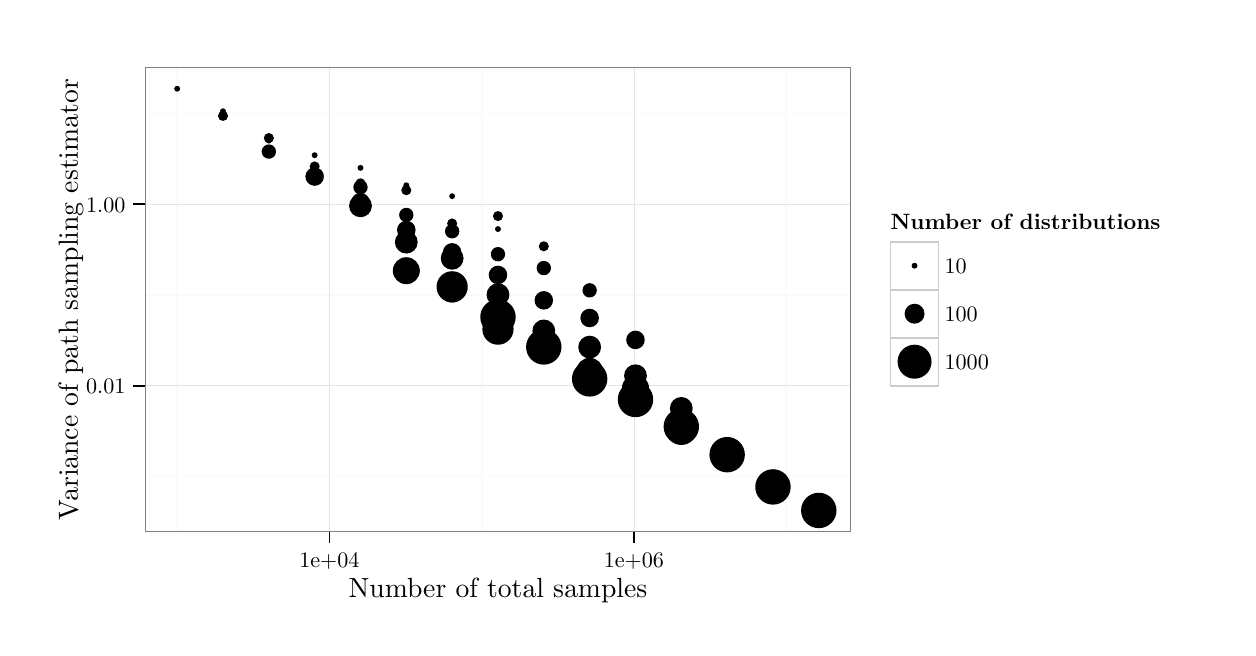
\begin{tikzpicture}[x=1pt,y=1pt]
\definecolor[named]{fillColor}{rgb}{1.00,1.00,1.00}
\path[use as bounding box,fill=fillColor,fill opacity=0.00] (0,0) rectangle (433.62,216.81);
\begin{scope}
\path[clip] (  0.00,  0.00) rectangle (433.62,216.81);
\definecolor[named]{drawColor}{rgb}{1.00,1.00,1.00}
\definecolor[named]{fillColor}{rgb}{1.00,1.00,1.00}

\path[draw=drawColor,line width= 0.6pt,line join=round,line cap=round,fill=fillColor] (  0.00,  0.00) rectangle (433.62,216.81);
\end{scope}
\begin{scope}
\path[clip] ( 42.43, 34.74) rectangle (297.46,202.36);
\definecolor[named]{fillColor}{rgb}{1.00,1.00,1.00}

\path[fill=fillColor] ( 42.43, 34.74) rectangle (297.46,202.36);
\definecolor[named]{drawColor}{rgb}{0.98,0.98,0.98}

\path[draw=drawColor,line width= 0.6pt,line join=round] ( 42.43, 54.67) --
	(297.46, 54.67);

\path[draw=drawColor,line width= 0.6pt,line join=round] ( 42.43,120.21) --
	(297.46,120.21);

\path[draw=drawColor,line width= 0.6pt,line join=round] ( 42.43,185.74) --
	(297.46,185.74);

\path[draw=drawColor,line width= 0.6pt,line join=round] ( 54.02, 34.74) --
	( 54.02,202.36);

\path[draw=drawColor,line width= 0.6pt,line join=round] (164.05, 34.74) --
	(164.05,202.36);

\path[draw=drawColor,line width= 0.6pt,line join=round] (274.07, 34.74) --
	(274.07,202.36);
\definecolor[named]{drawColor}{rgb}{0.90,0.90,0.90}

\path[draw=drawColor,line width= 0.2pt,line join=round] ( 42.43, 87.44) --
	(297.46, 87.44);

\path[draw=drawColor,line width= 0.2pt,line join=round] ( 42.43,152.98) --
	(297.46,152.98);

\path[draw=drawColor,line width= 0.2pt,line join=round] (109.03, 34.74) --
	(109.03,202.36);

\path[draw=drawColor,line width= 0.2pt,line join=round] (219.06, 34.74) --
	(219.06,202.36);
\definecolor[named]{fillColor}{rgb}{0.00,0.00,0.00}

\path[fill=fillColor] ( 54.02,194.74) circle (  1.07);

\path[fill=fillColor] ( 70.58,184.92) circle (  1.82);

\path[fill=fillColor] ( 87.14,172.03) circle (  2.59);

\path[fill=fillColor] (103.70,163.01) circle (  3.35);

\path[fill=fillColor] (120.26,152.43) circle (  4.12);

\path[fill=fillColor] (136.82,128.99) circle (  4.88);

\path[fill=fillColor] (153.38,123.16) circle (  5.64);

\path[fill=fillColor] (169.94,112.24) circle (  6.40);

\path[fill=fillColor] ( 70.58,186.62) circle (  1.07);

\path[fill=fillColor] ( 87.14,176.93) circle (  1.82);

\path[fill=fillColor] (103.70,163.63) circle (  2.59);

\path[fill=fillColor] (120.26,153.75) circle (  3.35);

\path[fill=fillColor] (136.82,139.31) circle (  4.12);

\path[fill=fillColor] (153.38,122.40) circle (  4.88);

\path[fill=fillColor] (169.94,107.88) circle (  5.64);

\path[fill=fillColor] (186.50,101.44) circle (  6.40);

\path[fill=fillColor] ( 87.14,176.01) circle (  1.07);

\path[fill=fillColor] (103.70,166.67) circle (  1.82);

\path[fill=fillColor] (120.26,159.14) circle (  2.59);

\path[fill=fillColor] (136.82,143.70) circle (  3.35);

\path[fill=fillColor] (153.38,133.47) circle (  4.12);

\path[fill=fillColor] (169.94,112.65) circle (  4.88);

\path[fill=fillColor] (186.50,100.95) circle (  5.64);

\path[fill=fillColor] (203.07, 89.90) circle (  6.40);

\path[fill=fillColor] (103.70,170.73) circle (  1.07);

\path[fill=fillColor] (120.26,160.57) circle (  1.82);

\path[fill=fillColor] (136.82,149.13) circle (  2.59);

\path[fill=fillColor] (153.38,135.62) circle (  3.35);

\path[fill=fillColor] (169.94,120.33) circle (  4.12);

\path[fill=fillColor] (186.50,100.42) circle (  4.88);

\path[fill=fillColor] (203.07, 90.48) circle (  5.64);

\path[fill=fillColor] (219.63, 82.46) circle (  6.40);

\path[fill=fillColor] (120.26,166.15) circle (  1.07);

\path[fill=fillColor] (136.82,158.07) circle (  1.82);

\path[fill=fillColor] (153.38,143.25) circle (  2.59);

\path[fill=fillColor] (169.94,127.45) circle (  3.35);

\path[fill=fillColor] (186.50,107.23) circle (  4.12);

\path[fill=fillColor] (203.07, 92.62) circle (  4.88);

\path[fill=fillColor] (219.63, 81.99) circle (  5.64);

\path[fill=fillColor] (236.19, 72.67) circle (  6.40);

\path[fill=fillColor] (136.82,159.86) circle (  1.07);

\path[fill=fillColor] (153.38,146.06) circle (  1.82);

\path[fill=fillColor] (169.94,134.95) circle (  2.59);

\path[fill=fillColor] (186.50,118.28) circle (  3.35);

\path[fill=fillColor] (203.07,101.38) circle (  4.12);

\path[fill=fillColor] (219.63, 86.59) circle (  4.88);

\path[fill=fillColor] (236.19, 71.66) circle (  5.64);

\path[fill=fillColor] (252.75, 62.51) circle (  6.40);

\path[fill=fillColor] (153.38,155.91) circle (  1.07);

\path[fill=fillColor] (169.94,148.73) circle (  1.82);

\path[fill=fillColor] (186.50,129.94) circle (  2.59);

\path[fill=fillColor] (203.07,111.90) circle (  3.35);

\path[fill=fillColor] (219.63, 91.03) circle (  4.12);

\path[fill=fillColor] (236.19, 74.85) circle (  4.88);

\path[fill=fillColor] (252.75, 61.94) circle (  5.64);

\path[fill=fillColor] (269.31, 50.86) circle (  6.40);

\path[fill=fillColor] (169.94,144.04) circle (  1.07);

\path[fill=fillColor] (186.50,137.81) circle (  1.82);

\path[fill=fillColor] (203.07,121.90) circle (  2.59);

\path[fill=fillColor] (219.63,103.99) circle (  3.35);

\path[fill=fillColor] (236.19, 79.23) circle (  4.12);

\path[fill=fillColor] (252.75, 62.57) circle (  4.88);

\path[fill=fillColor] (269.31, 50.50) circle (  5.64);

\path[fill=fillColor] (285.87, 42.36) circle (  6.40);
\definecolor[named]{drawColor}{rgb}{0.50,0.50,0.50}

\path[draw=drawColor,line width= 0.6pt,line join=round,line cap=round] ( 42.43, 34.74) rectangle (297.46,202.36);
\end{scope}
\begin{scope}
\path[clip] (  0.00,  0.00) rectangle (433.62,216.81);
\definecolor[named]{drawColor}{rgb}{0.00,0.00,0.00}

\node[text=drawColor,anchor=base east,inner sep=0pt, outer sep=0pt, scale=  0.80] at ( 35.32, 84.51) {0.01};

\node[text=drawColor,anchor=base east,inner sep=0pt, outer sep=0pt, scale=  0.80] at ( 35.32,150.05) {1.00};
\end{scope}
\begin{scope}
\path[clip] (  0.00,  0.00) rectangle (433.62,216.81);
\definecolor[named]{drawColor}{rgb}{0.00,0.00,0.00}

\path[draw=drawColor,line width= 0.6pt,line join=round] ( 38.16, 87.44) --
	( 42.43, 87.44);

\path[draw=drawColor,line width= 0.6pt,line join=round] ( 38.16,152.98) --
	( 42.43,152.98);
\end{scope}
\begin{scope}
\path[clip] (  0.00,  0.00) rectangle (433.62,216.81);
\definecolor[named]{drawColor}{rgb}{0.00,0.00,0.00}

\path[draw=drawColor,line width= 0.6pt,line join=round] (109.03, 30.47) --
	(109.03, 34.74);

\path[draw=drawColor,line width= 0.6pt,line join=round] (219.06, 30.47) --
	(219.06, 34.74);
\end{scope}
\begin{scope}
\path[clip] (  0.00,  0.00) rectangle (433.62,216.81);
\definecolor[named]{drawColor}{rgb}{0.00,0.00,0.00}

\node[text=drawColor,anchor=base,inner sep=0pt, outer sep=0pt, scale=  0.80] at (109.03, 21.77) {1e+04};

\node[text=drawColor,anchor=base,inner sep=0pt, outer sep=0pt, scale=  0.80] at (219.06, 21.77) {1e+06};
\end{scope}
\begin{scope}
\path[clip] (  0.00,  0.00) rectangle (433.62,216.81);
\definecolor[named]{drawColor}{rgb}{0.00,0.00,0.00}

\node[text=drawColor,anchor=base,inner sep=0pt, outer sep=0pt, scale=  1.00] at (169.94, 10.84) {Number of total samples};
\end{scope}
\begin{scope}
\path[clip] (  0.00,  0.00) rectangle (433.62,216.81);
\definecolor[named]{drawColor}{rgb}{0.00,0.00,0.00}

\node[text=drawColor,rotate= 90.00,anchor=base,inner sep=0pt, outer sep=0pt, scale=  1.00] at ( 18.16,118.55) {Variance of path sampling estimator};
\end{scope}
\begin{scope}
\path[clip] (  0.00,  0.00) rectangle (433.62,216.81);
\definecolor[named]{fillColor}{rgb}{1.00,1.00,1.00}

\path[fill=fillColor] (307.53, 83.17) rectangle (409.09,153.93);
\end{scope}
\begin{scope}
\path[clip] (  0.00,  0.00) rectangle (433.62,216.81);
\definecolor[named]{drawColor}{rgb}{0.00,0.00,0.00}

\node[text=drawColor,anchor=base west,inner sep=0pt, outer sep=0pt, scale=  0.80] at (311.80,143.81) {\bfseries Number of distributions};
\end{scope}
\begin{scope}
\path[clip] (  0.00,  0.00) rectangle (433.62,216.81);
\definecolor[named]{drawColor}{rgb}{0.80,0.80,0.80}
\definecolor[named]{fillColor}{rgb}{1.00,1.00,1.00}

\path[draw=drawColor,line width= 0.6pt,line join=round,line cap=round,fill=fillColor] (311.80,122.13) rectangle (329.14,139.47);
\end{scope}
\begin{scope}
\path[clip] (  0.00,  0.00) rectangle (433.62,216.81);
\definecolor[named]{fillColor}{rgb}{0.00,0.00,0.00}

\path[fill=fillColor] (320.47,130.80) circle (  1.07);
\end{scope}
\begin{scope}
\path[clip] (  0.00,  0.00) rectangle (433.62,216.81);
\definecolor[named]{drawColor}{rgb}{0.80,0.80,0.80}
\definecolor[named]{fillColor}{rgb}{1.00,1.00,1.00}

\path[draw=drawColor,line width= 0.6pt,line join=round,line cap=round,fill=fillColor] (311.80,104.78) rectangle (329.14,122.13);
\end{scope}
\begin{scope}
\path[clip] (  0.00,  0.00) rectangle (433.62,216.81);
\definecolor[named]{fillColor}{rgb}{0.00,0.00,0.00}

\path[fill=fillColor] (320.47,113.45) circle (  3.60);
\end{scope}
\begin{scope}
\path[clip] (  0.00,  0.00) rectangle (433.62,216.81);
\definecolor[named]{drawColor}{rgb}{0.80,0.80,0.80}
\definecolor[named]{fillColor}{rgb}{1.00,1.00,1.00}

\path[draw=drawColor,line width= 0.6pt,line join=round,line cap=round,fill=fillColor] (311.80, 87.44) rectangle (329.14,104.78);
\end{scope}
\begin{scope}
\path[clip] (  0.00,  0.00) rectangle (433.62,216.81);
\definecolor[named]{fillColor}{rgb}{0.00,0.00,0.00}

\path[fill=fillColor] (320.47, 96.11) circle (  6.14);
\end{scope}
\begin{scope}
\path[clip] (  0.00,  0.00) rectangle (433.62,216.81);
\definecolor[named]{drawColor}{rgb}{0.00,0.00,0.00}

\node[text=drawColor,anchor=base west,inner sep=0pt, outer sep=0pt, scale=  0.80] at (331.31,127.87) {10};
\end{scope}
\begin{scope}
\path[clip] (  0.00,  0.00) rectangle (433.62,216.81);
\definecolor[named]{drawColor}{rgb}{0.00,0.00,0.00}

\node[text=drawColor,anchor=base west,inner sep=0pt, outer sep=0pt, scale=  0.80] at (331.31,110.53) {100};
\end{scope}
\begin{scope}
\path[clip] (  0.00,  0.00) rectangle (433.62,216.81);
\definecolor[named]{drawColor}{rgb}{0.00,0.00,0.00}

\node[text=drawColor,anchor=base west,inner sep=0pt, outer sep=0pt, scale=  0.80] at (331.31, 93.18) {1000};
\end{scope}
\end{tikzpicture}

\end{document}
